
\documentclass[twocolumn,10pt]{article}

\usepackage{epsfig} %% for loading postscript figures
%\usepackage[
%backend=biber,
%style=alphabetic,
%citestyle=authoryear
%]{biblatex}
\usepackage{hyperref}
\usepackage{natbib}
\usepackage{amsmath}
\usepackage{graphicx}
\DeclareMathOperator*{\argmax}{arg\,max}
\DeclareMathOperator*{\argmin}{arg\,min}

\title{Neural Machine Translation}

%%% first author
\author{Srujan \\Netid:ssg7}

\begin{document}

\maketitle

Machine translation refers to automatic translation of a word, phrase, sentence or text of one language into another by a machine with minimal human intervention. Machine translation goes beyond a mere word-to-word substitution between the language pair. Some language pairs can be translated with minimal effort owing to their similar syntactical rules while most pairs don't have that luxury. Models to construct machine translation systems have evolved over the years and widely fall into four categories: Rule-based, Statistical, Hybrid and Neural models. After a short description of all the models, this tech review delves into Neural Machine Translation models and their state-of-the-art. 

%%%%%%%%%%%%%%%%%%%%%%%%%%%%%%%%%%%%%%%%%%%%%%%%%%%%%%%%%%%%%%%%%%%%%%
\section{Machine Translation models}
\subsection{Rule-based Machine Translation}
As the name suggests, RBMT is heavily language-pair dependent. Constructing an RBMT model involves an in-depth understanding and builidng of grammar rules of languages in question. RBMT also uses a dictionary/lexicon for word substition. A rudimentary model involves processing an input text and conducting syntax identification, semantic analysis, and POS tagging. Then comes mapping the primary language's syntactical structure to that of the target language and finally substituting the primary language's words with the dictionary entries of the target language. RBMT is robust in that if a language pair is well mapped, translations are often very accurate. Hand debugging makes it very easy to incorporate exceptions to the rules and general mapping. RBMTs typically involve a lot of human effort to build and/or expand. There are several other shortcomings that make them less scalable across multiple languages. Open source projects like Apertium\cite{apertium} are still available to use.  
\subsection{Statistical Machine Translation}
Statistical Machine Translation is a data driven approach unlike RBMT. Similar to a feedback model in Information Retrieval, SMT assumes there exists a counterpart sentence, phrase or word in the primary language with a certain probability that maps to a corresponding sentence, phrase or word in target language\cite{kit} . So, if \(P(t)\) is the probability of a target language, and \(P(t|s)\) is the conditional probabilty of target language given a primary language input, we use naive Baye's to find a t such that: \[t=\argmax P(t|s)*P(t)\]
\par
Because it heavily depends on probability of occurrence of a phrase, SMT performs poorly when translating obscure phrases or syntactically correct yet awkwardly constructed sentences. \cite{genzel} particularly explores how SMT should be modified to be able to translate poetry while maintaining the rhyme, meter and perhaps the tone. 
\subsection{Hybrid Machine Translation}
Hybrid Machine Translation model combines the advantages of Rule-based and Statistical models to improve the quality of translation. The combinations can be done in multiple ways, but \cite{xuan} describes an interesting serial model that first uses RBMT to translate and then uses SMT to replace a part of RBMT's output based on bilingual trained SMT model. Other implementations involing using RBMT after an SMT output are also conceived.  
\subsection{Neural Machine Translation}
As the name suggests, NMT employs neural networks to achieve translation as opposed to elaborate rule based syntactical approaches. An NMT, in effect, mimics a human brain, with apriori bilingual knowledge, that listens to a phrase or sentence and translates. Neural Machine Translation models often don't require a sentence to be broken down into sub units for processing unlike all the other models. Several open source tools exist to implement Neural Machine Translation models. This tech review delves deeper into a popular open source NMT tool called seq2seq. The review also touches on other tools briefly.
\subsubsection{Seq2Seq}
The structure of this model has an encoder-decoder architecture. The encoder accepts a sentence for e.g. `` I am a student'' and the translation output from decoder should be ``Je suis \'etudient''. 
\begin{figure}[h]
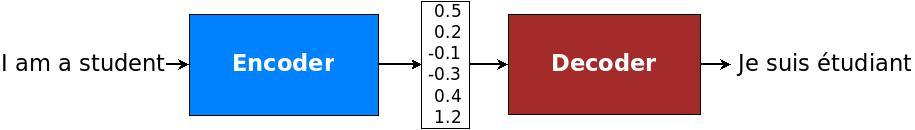
\includegraphics[width=0.5\textwidth]{encdec.jpg}
\caption{Encoder, Transformed vector, Decoder architecture\cite{NMTtut}}
\label{fig:encdec}
\end{figure}
\par
The seq2seq model uses a multi layer Recurrent Neural Network (RNN). Using the example quoted in \ref{fig:encdec}, this NMT model has two RNNs one for encoder and another for decoder.
\par
The RNNs are trained using English - French embeddings of the sentences ``I am a student'' and ``Je suis \'etudient'' as described in \cite{NMTtut}. Using a suitable optimizer like gradient descdent, the weight are updated via backpropogation (typically). Once trained, the RNNs can be used for inference and generating translations for new sentences.
\subsubsection{GNMT}
Google's Neural Machine Translation which was recently deployed replaced its old Phrase based Machine Translation which was a statistical machine translation technique. GNMT uses a similar structure as that of seq2seq model described above. Although, Google makes use of their massive parallel architectures called Tensor Processing Units(TPUs) to exploit the parallel nature of training RNNs. GNMT reports an error reduction of 55-85 \% for major language pairs\cite{goog}.

\bibliographystyle{plain}
\bibliography{sample} 


\end{document}
